\documentclass[conference]{IEEEtran}
\usepackage[utf8]{inputenc}
\usepackage{amsmath,amssymb}
\usepackage{graphicx}
\usepackage{booktabs}
\usepackage{siunitx}
\usepackage{tikz}
\usetikzlibrary{positioning,arrows.meta,fit}
\usepackage[hidelinks]{hyperref}
\usepackage{cite}

\sisetup{detect-all, range-phrase = --, range-units = single, uncertainty-mode = separate}
\newcommand{\degr}{\ensuremath{^\circ}}

\begin{document}

\title{Autonomous Drift Parking with Lidar and\\ Nonlinear MPC on a 1:10 Ackermann Car}

\author{\IEEEauthorblockN{Pietro Gelmini}
\IEEEauthorblockA{University of Trento, Italy\\
gelmini.pietro@gmail.com}}

\maketitle


\begin{abstract}
A 1:10 Ackermann car with hard plastic tires parks itself sideways between two boxes on a tiled floor, drifting
into gaps as short as \SI{47}{cm}, 1.8 times its length. Its dynamics were identified from an overhead
camera, an IMU and the wheel encoders: a single-track model with saturating tires and a spool rear axle. On it a
nonlinear model predictive controller (NMPC, acados) runs on the car's Raspberry Pi~4 at \SI{50}{Hz} and holds a
tight line where Pure Pursuit cuts the corners, or spins on a slippery floor in simulation. A first goal, holding a
sustained drift around a cone, worked in simulation and failed on the car: the drift the controller held is an
unstable equilibrium of the model that the real car does not keep. The final manoeuvre uses the regime where the
model is right, the slide with the rear wheels locked: the lidar measures the gap, the car kicks into a drift at
full lock, and the brake is timed on the gyro so that the slide ends at \SI{180}{\degree}. Over nine runs the car
stopped at \SI{180.8 \pm 2.9}{\degree}. It also parks between boxes placed anywhere in a mapped room, planning and
driving the approach with the NMPC, and runs a one-take gymkhana (slalom, donut, parking), ten clean takes on the day it was filmed.
The same software runs unchanged in a Gazebo twin of the car and the room.
\end{abstract}

\section{Introduction}

Driving at the limit of tire friction is where vehicle control is both hardest and most needed: emergency
manoeuvres on ice, racing, recovery from a slide. Full-scale research platforms have shown controlled drifting
along general paths~\cite{hindiyeh2014,goh2020} and autonomous sliding into a parking spot~\cite{kolter2010}.
Small-scale cars make such experiments cheap and safe~\cite{liniger2015,okelly2020,cutler2016}, but they move the
difficulty elsewhere: tires that are hard and poorly characterized, low-rate sensors, and all computation on a
single-board computer.

\begin{figure}[t]
\centering
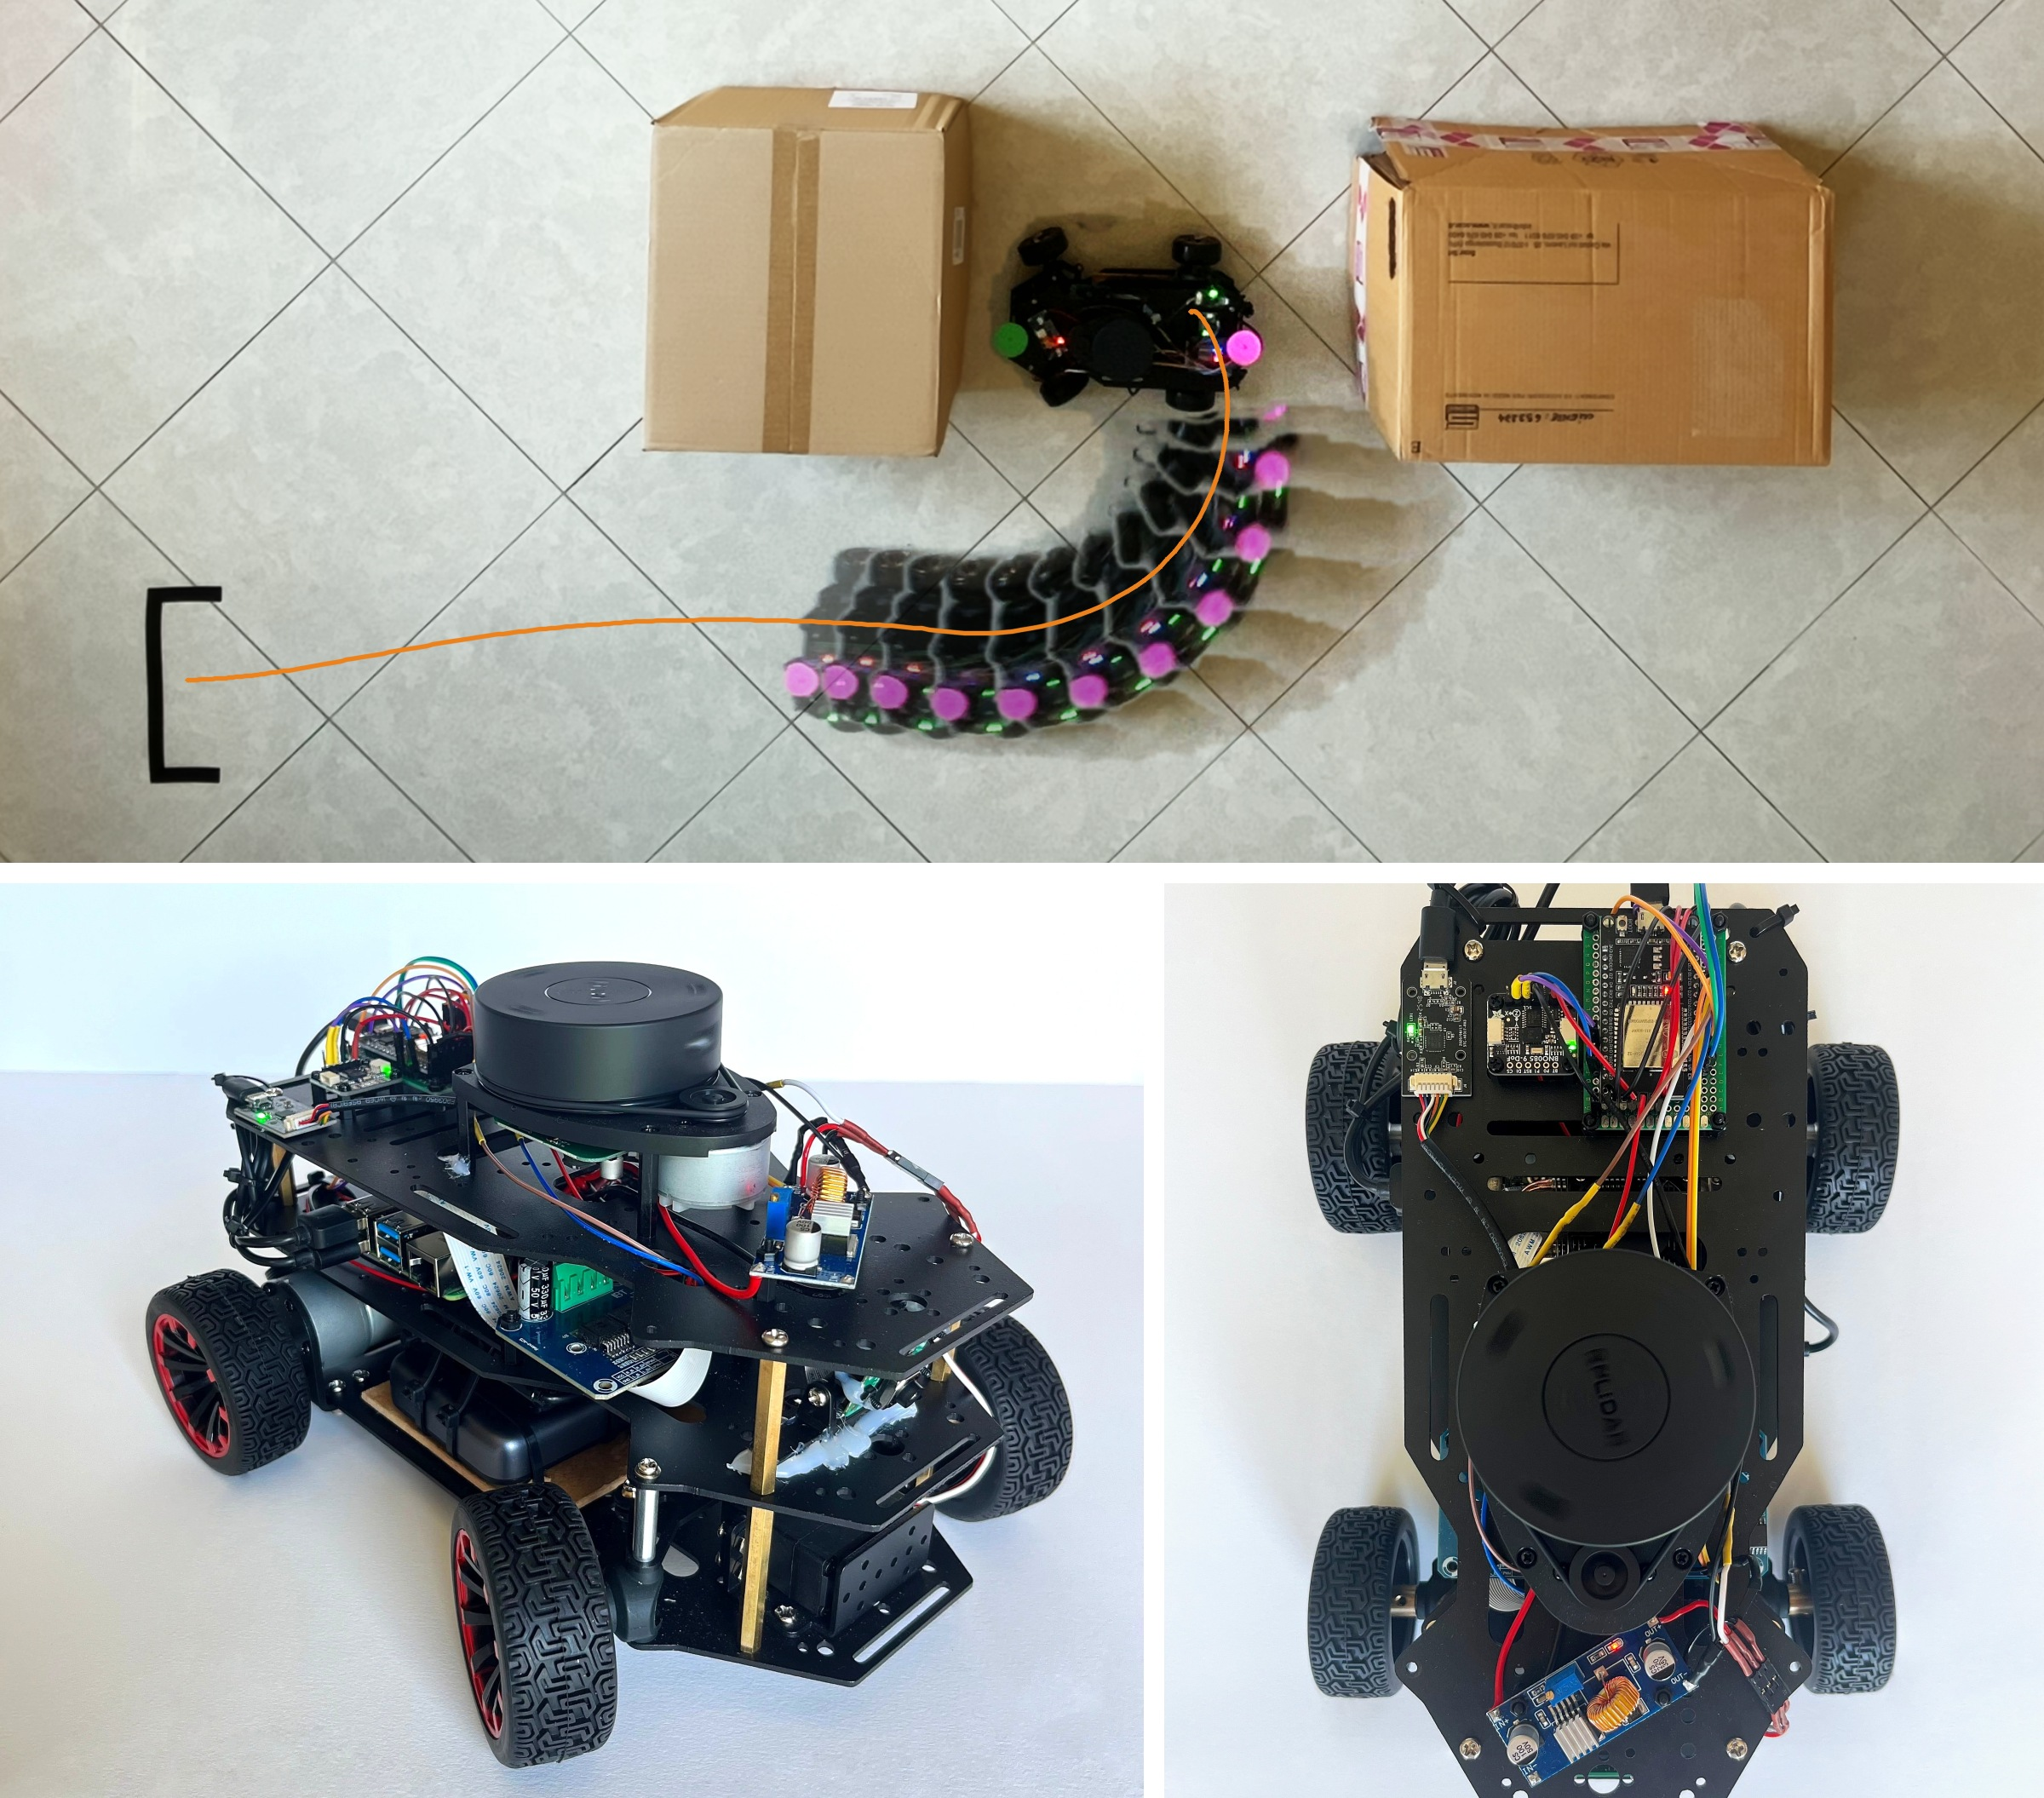
\includegraphics[width=\columnwidth]{figures/hero.jpg}
\caption{Top: the car parking itself into a \SI{47}{cm} gap, seen by an overhead camera; the car every \SI{0.1}{s}
from the kick to the stop, and the path of its rear axle from the start mark (left). Bottom: the car,
\SI{0.26}{m} long and \SI{2.0}{kg}, with the lidar on top.}
\label{fig:hero}
\end{figure}

This report describes a complete stack on a car built for about 510 euros, from the identification of its
dynamics to autonomous manoeuvres beyond the limit of grip, including one that did not work. The contributions are:
\begin{itemize}
\item an identified dynamic model of a 1:10 car with a spool rear axle and saturating tires, from overhead video,
  IMU and encoders, refitted for locked-wheel slides on lidar ground truth (Sec.~\ref{sec:model});
\item an NMPC on that model running on the car's Raspberry Pi~4 at \SI{50}{Hz}, tested against Pure Pursuit on
  the car and, at lower friction, in simulation (Sec.~\ref{sec:nmpc});
\item a negative result on sustained drifting: the drift that the controller holds in simulation is an unstable
  steady state of the model that the real car does not have (Sec.~\ref{sec:drift});
\item drift parking: sideways into a lidar-measured gap of 1.8 car lengths, between boxes placed anywhere in a
  room, and a one-take gymkhana (Sec.~\ref{sec:parking}, \ref{sec:anywhere});
\item a Gazebo twin running the identical software stack (Sec.~\ref{sec:sim}).
\end{itemize}
Code, notebooks with every analysis, and the video are at
\url{https://github.com/Gelminaio/drift-mpc-ackermann}.


\section{Platform}

The car (Fig.~\ref{fig:hero}) is a 1:10 Ackermann chassis with servo steering and a rear axle driven as a spool by
two geared DC motors with quadrature encoders (660 ticks per revolution) through BTS7960 half bridges. It weighs
\SI{2.015}{kg}, \SI{57}{\percent} on the rear axle, with a wheelbase of \SI{0.173}{m}. Hard plastic drift tires on
tiles slide at a friction coefficient of about 0.25--0.28 at the rear. The steering reaches
\SI{28.9}{\degree} to the left and \SI{21.8}{\degree} to the right; the motors limit the wheel speed to
\SI{1.2}{m/s}.

Two computers share the work (Fig.~\ref{fig:arch}). An ESP32 runs the real-time layer under FreeRTOS: wheel speed
PID control at \SI{100}{Hz}, encoders, a BNO085 IMU, the servo, and a safety supervisor (arming, command timeout,
stall detection, watchdog). It talks micro-ROS over USB serial and stamps its messages on the clock of the
Raspberry Pi~4, where they arrive \SI{7}{ms} old. A speed setpoint of zero shorts the motor: the rear wheels lock
within \SIrange{0.35}{0.4}{s}, which is the handbrake of Sec.~\ref{sec:parking}. The Pi runs ROS~2
Jazzy~\cite{ros2}: the RPLIDAR A1 driver (\SI{6.8}{Hz}), wheel odometry, an EKF on wheel speed and gyro
(robot\_localization~\cite{moore2014}), AMCL~\cite{fox1999} on an occupancy map of the room (first from
slam\_toolbox~\cite{macenski2021}, later rebuilt from registered scans), and the controllers. A desktop runs only the simulation and the analysis. Measured against the encoder count, the lidar
scan is \SIrange{56}{76}{ms} old when it arrives and the gyro \SIrange{44}{64}{ms}; the controllers carry the
state forward over these delays.

\begin{figure}[t]
\centering
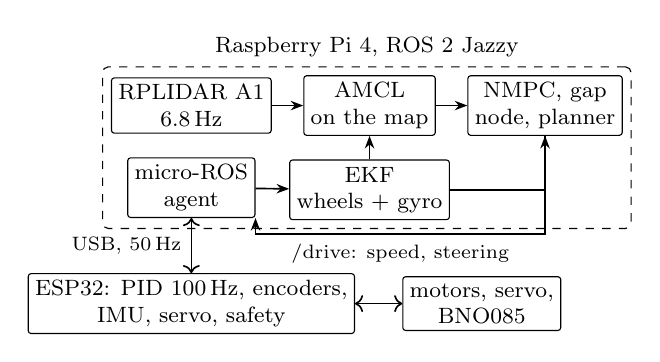
\begin{tikzpicture}[font=\footnotesize, node distance=3mm and 4mm,
  blk/.style={draw, rounded corners=1pt, align=center, inner sep=2.5pt, minimum height=5mm},
  grp/.style={draw, dashed, rounded corners=2pt, inner sep=3pt},
  arr/.style={-{Stealth[length=1.6mm]}, semithick}]
\node[blk] (lidar) {RPLIDAR A1\\ \SI{6.8}{Hz}};
\node[blk, right=of lidar] (amcl) {AMCL\\ on the map};
\node[blk, right=of amcl] (ctrl) {NMPC, gap\\ node, planner};
\node[blk, below=of amcl] (ekf) {EKF\\ wheels + gyro};
\node[blk, below=of lidar] (agent) {micro-ROS\\ agent};
\node[grp, fit=(lidar)(amcl)(ctrl)(ekf)(agent), label={[font=\footnotesize]above:Raspberry Pi 4, ROS 2 Jazzy}] (pi) {};
\node[blk, below=7mm of agent] (esp) {ESP32: PID \SI{100}{Hz}, encoders,\\ IMU, servo, safety};
\node[blk, right=6mm of esp] (car) {motors, servo,\\ BNO085};
\draw[arr] (lidar) -- (amcl);
\draw[arr] (amcl) -- (ctrl);
\draw[arr] (ekf) -- (amcl);
\draw[arr] (ekf) -| (ctrl);
\draw[arr] (agent) -- (ekf);
\draw[arr, <->] (agent) -- node[left, font=\scriptsize] {USB, \SI{50}{Hz}} (esp);
\draw[arr, <->] (esp) -- (car);
\draw[arr] (ctrl.south) |- ++(0,-1.25) -| node[pos=0.25, below, font=\scriptsize] {/drive: speed, steering} (agent.south east);
\end{tikzpicture}
\caption{Hardware and software. Everything runs on the car; the same nodes run in Gazebo against a plugin that
replaces the ESP32 and the car.}
\label{fig:arch}
\end{figure}

\section{Model and identification}\label{sec:model}

\subsection{Single-track model}

The body velocities $v_x, v_y$ and yaw rate $r$ are those of the centre of gravity (CG), with $l_f$ and $l_r$ its
distances to the axles and $T$ the track. The front axle is one tire at slip angle
$\alpha_f = \delta - \arctan\big((v_y + l_f r)/v_x\big)$,
\begin{equation}
F_{yf} = \mu_f N_f \sin\!\big(C \arctan(B_f \alpha_f)\big),
\end{equation}
a simplified magic formula~\cite{pacejka2012}. The rear is a spool: both wheels turn at the same surface speed $u$
and each slides over the ground at its own velocity $(v_{x,i}, v_{y,i}) = (v_x \mp \tfrac{T}{2} r,\, v_y - l_r r)$.
With the slip vector $\boldsymbol{\sigma}_i = (v_{x,i} - u,\; v_{y,i})/u$, each rear tire pushes against its own
sliding direction,
\begin{equation}
\mathbf{F}_i = -\frac{\mu_r N_r}{2} \sin\!\big(C \arctan(B_r |\boldsymbol{\sigma}_i|)\big)
\frac{\boldsymbol{\sigma}_i}{|\boldsymbol{\sigma}_i|},
\end{equation}
sideways in a turn, forward when the wheels spin, backward when they are locked. The steering angle follows its
command through a first-order lag $\tau_\delta$ and the wheel speed follows its setpoint through the motor control
loop. A floor with a different friction is a scale $k$ on the peak forces, $\mu \to k\mu$ and $B \to B/k$, which
keeps the cornering stiffness: the brush model's behaviour~\cite{pacejka2012}.

\subsection{Identification}

Geometry and mass were measured directly, the CG from the axle loads on a level and a tilted car, the yaw inertia
with a bifilar pendulum~\cite{jardin2009}: $I_z = \SI{0.0125}{kg\,m^2} \pm \SI{2.3}{\percent}$. For the dynamics,
a phone \SI{2}{m} above the floor filmed the car with two coloured markers \SI{267}{mm} apart on its centre line; the
markers give position, heading and, with the encoders, the CG velocity and sideslip, aligned with the bag on the
yaw rate. Steering steps, a steering chirp (\SIrange{0.2}{2.5}{Hz}), a drift entry and exit, and a steering release
inside the drift were each driven twice, one run to fit and one to validate. The five tire parameters and
$\tau_\delta$ were fitted by least squares on yaw rate and sideslip over the three identification runs together,
so that one parameter set covers grip and drift (Table~\ref{tab:params}).

The fit has $C < 1$: the tire curves rise to $\mu N \sin(C\pi/2)$ and stay there, with no peak. At full slide the
rear gives 0.276, against 0.248 from straight launches with wheelspin, an independent test. The steering lag is
\SI{0.17}{s}, against \SIrange{25}{40}{ms} for the servo alone on a stand: most of it lies between the wheel angle and
the tire force. Predicting \SI{1}{s} ahead from the measured state, the way the NMPC uses the model, the yaw rate is
within an NRMSE of 11--17\% on the validation runs, the sideslip within \SIrange{1.4}{1.6}{\degree} in grip and
\SIrange{3.1}{3.9}{\degree} in the drift (Fig.~\ref{fig:ident}).

For the locked-wheel slides of Sec.~\ref{sec:parking} the model was refitted on a second ground truth: the path of
the rear axle from the lidar, every scan registered by ICP~\cite{besl1992} on the scans taken at rest, each beam
moved to where the car was when it was taken (\SIrange{0.9}{1.3}{cm} rms per scan). The refit adds lateral and
longitudinal load transfer and, while braked, separate rear friction factors along and across the wheel; it asks
for a locked rear that slides with 1.37 times the friction along the wheel and 0.94 times across it. Over
held-out windows of \SI{1.2}{s} the refit ends \SIrange{2.4}{6.2}{cm} off, against \SIrange{4.5}{7.2}{cm} for the
first model.

\begin{table}[t]
\caption{Identified parameters}
\label{tab:params}
\centering
\footnotesize
\begin{tabular}{@{}llr@{}}
\toprule
mass; yaw inertia & $m$; $I_z$ & \SI{2.015}{kg}; \SI{0.0125}{kg\,m^2} \\
CG to the axles; height & $l_f$, $l_r$; $h$ & 98.6, 74.4; \SI{67}{mm} \\
track; wheel radius & $T$; $R_w$ & 174.5; \SI{29.9}{mm} \\
front tire & $\mu_f$, $B_f$ & 0.449, 60 \\
rear tire & $\mu_r$, $B_r$ & 0.315, 20.8 \\
shape factor & $C$ & 0.678 \\
full slide, front; rear & $\mu \sin(C\pi/2)$ & 0.393; 0.276 \\
steering lag; servo rate & $\tau_\delta$ & \SI{0.169}{s}; \SI{250}{\degree/s} \\
wheel speed lag; top speed & & \SIrange{15}{45}{ms}; \SI{1.2}{m/s} \\
\bottomrule
\end{tabular}
\end{table}

\begin{figure}[t]
\centering
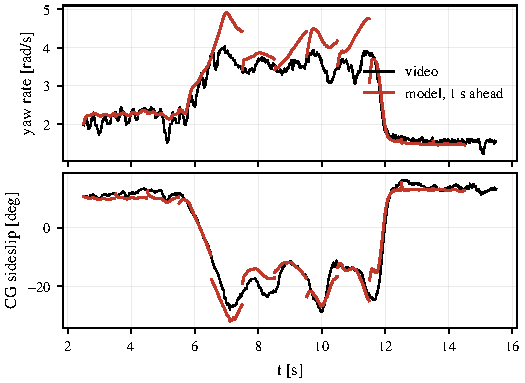
\includegraphics[width=\columnwidth]{figures/ident.pdf}
\caption{The model \SI{1}{s} ahead from the measured state, restarted every second, against the overhead video
on the validation drift run: cornering at \SI{0.9}{m/s}, the drift at full throttle, back to grip.}
\label{fig:ident}
\end{figure}

\section{Nonlinear MPC at the limit}\label{sec:nmpc}

\subsection{Problem}

The NMPC tracks a path with the rear axle rather than the CG. In grip the rear axle moves along the car's heading,
so a heading error of zero means the car is aligned with the path; tracking the CG instead, which slides by
\SIrange{5}{7}{\degree} in a corner, made the controller lock the rear wheels to rotate the car. The state is
\begin{equation}
x = (s,\, n,\, e_\psi,\, v_x,\, v_y,\, r,\, \delta,\, u,\, \delta_c,\, u_c),
\end{equation}
progress $s$, lateral offset $n$ and heading error $e_\psi$ of the rear axle to the path, the body states, the
steering angle and wheel speed, and the two commands sent to the car. The inputs are the command rates, bounded by
the servo (\SI{4.36}{rad/s}) and by \SI{5}{m/s^2}; the commands are bounded by the steering map and
\SIrange{0}{1.2}{m/s}. With path curvature $\kappa(s)$ and the lateral velocity of the rear axle
$v_{y,r} = v_y - l_r r$,
\begin{align}
\dot s &= \frac{v_x \cos e_\psi - v_{y,r} \sin e_\psi}{1 - n\kappa}, &
\dot n &= v_x \sin e_\psi + v_{y,r} \cos e_\psi, \nonumber\\
\dot e_\psi &= r - \kappa \dot s,
\end{align}
with the body dynamics of Sec.~\ref{sec:model}. The cost is a weighted sum of $n$ (\SI{5}{cm}), $e_\psi$
(\SI{0.1}{rad}), the speed error against a profile (\SI{0.3}{m/s}) and the command rates; $|n| < \SI{0.3}{m}$ and
$v_x > \SI{0.3}{m/s}$ are soft constraints. There is no bound on the tire slip: the tires may saturate.

The horizon is \SI{1}{s} in 25 stages, 10 of \SI{20}{ms} and 15 of \SI{53}{ms}. acados~\cite{acados2022} generates
the solver from the CasADi~\cite{casadi2019} model: an implicit Gauss--Legendre integrator~\cite{hairer1996} (the
front tire makes the model stiff at low speed, where explicit RK4 needs steps under \SI{4}{ms}), one Gauss--Newton SQP
iteration per control step in the spirit of the real-time iteration~\cite{diehl2005}, HPIPM~\cite{hpipm2020} for
the QP, and a merit-function line search. The plain full step overshoots where the tires saturate: the steering
chattered on 25--38\% of the steps. A \SI{50}{Hz} horizon of 50 stages took \SI{10.5}{ms} on the Pi;
the split horizon takes \SI{5.6}{ms} on average and \SI{9.6}{ms} at worst with the whole stack running. The C++
node publishes a command every \SI{20}{ms}; on the car it solved in \SI{8}{ms} on average and exceeded the step once
in 1548.

\subsection{Results}

Table~\ref{tab:nmpc} compares the NMPC with Pure Pursuit~\cite{coulter1992}, tuned on the same model with a
delayed pose. In a Python closed loop on the true state the NMPC halves the error and holds the line at 120\% of
the grip a speed profile assumes, where Pure Pursuit spins. In Gazebo with the full stack and the friction scaled,
Pure Pursuit spins in the first lap at 25\% of the grip of the tiles while the NMPC drives three laps,
\SI{10}{\percent} slower (Fig.~\ref{fig:nmpc}). On the car, on a line with \SI{0.4}{m} corners driven at full speed,
the NMPC stays \SI{2.7}{cm} rms from it against \SI{7.1}{cm}: Pure Pursuit cuts the corners, its lookahead being
longer than their arcs. On a wider line the two are even (\SI{3.5}{cm} against \SI{3.4}{cm}), and there the error
is the localization's: about \SI{6}{cm} rms against the ground truth in Gazebo, and the NMPC, which steers twice as
much as Pure Pursuit, chases it.

\begin{table}[t]
\caption{Rear axle off the line, rms (max) [cm]: Python closed loop on the true state, Gazebo with the whole stack
against the true path, the car against its localization}
\label{tab:nmpc}
\centering
\footnotesize
\begin{tabular}{@{}llrr@{}}
\toprule
& floor; line & Pure Pursuit & NMPC \\
\midrule
Python & tiles & 3.2 (6.8) & 1.6 (3.1) \\
& 25\% grip, profile at 120\% & spins & 1.8 (4.5) \\
Gazebo & 35\% grip & 7.6 (28) & 3.3 (8) \\
& 25\% grip & spins & 6.7 (18) \\
car & tiles; \SI{0.4}{m} corners & 7.1 (19.4) & 2.7 (7.4) \\
& tiles; \SI{0.6}{m} corners & 3.4 (8.5) & 3.5 (7.1) \\
\bottomrule
\end{tabular}
\end{table}

\begin{figure*}[t]
\centering
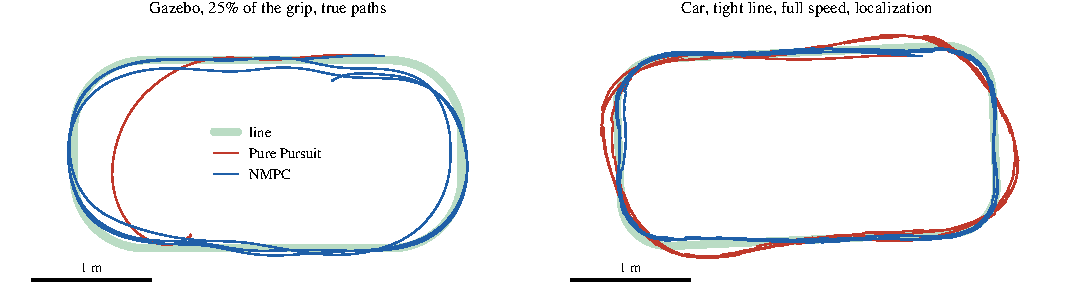
\includegraphics[width=\textwidth]{figures/nmpc.pdf}
\caption{Left: Gazebo at 25\% of the grip of the tiles, true paths; Pure Pursuit spins in the first lap. Right:
the car on the tight line at full speed, paths from its localization.}
\label{fig:nmpc}
\end{figure*}

\section{Drift around a cone: a negative result}\label{sec:drift}

With the steering and the wheel speed held, the model has up to three steady states~\cite{velenis2010}: grip, a
saddle, and a drift. The drift is stable on its own because the firmware holds the wheel speed, and with it the
rear slip; it matches the donut of the identification runs (\SI{0.49}{m/s}, \SI{-18}{\degree} of sideslip at the
CG against the measured \SI{0.50}{m/s} and \SI{-18}{\degree} to \SI{-21}{\degree}). These stable drifts are tight,
\SIrange{11}{19}{cm} of CG radius, too tight for a cone at the centre. The goal of a drift around a cone was a wider,
unstable equilibrium (\SI{13}{\degree} of steering, \SI{1.12}{m/s} at the wheels, \SI{0.27}{m} of radius and
\SI{-25}{\degree} of rear slip) held by an NMPC with the same model and solver, its reference the cone in the
lidar scan.

In Gazebo it worked: the rear axle held \SI{28.8 \pm 0.1}{cm} from the cone against \SI{28.9}{cm}, within
\SI{1.1}{cm} with the scan delivered \SI{0.15}{s} late as on the real lidar. Since the state on the circle is
known, the steady-state force balance also gives the friction of the floor: on five floors from 0.90 to 1.10
times the tiles the estimate ended within \SI{0.6}{\percent}.

On the car the drift never held for more than \SI{0.5}{s} (Fig.~\ref{fig:drift}). The rear let go only on a torque
step at full lock, never under the rate-limited commands of the NMPC; once sliding, any correction, a little less
steering or a little less speed, gripped it again within \SIrange{0.25}{0.5}{s}. Open loop, opening the steering
from the donut at full throttle, the car keeps sliding only from \SI{16}{\degree}, on a \SI{0.19}{m} circle; at
\SIrange{12}{14}{\degree} it fades back to grip. The tight stable drifts exist on the car as in the model; the
unstable middle state the simulator held does not. The model's rear tire loses grip too easily at moderate
longitudinal slip, which places the unstable equilibrium where the car has none. The work moved to the one regime
where the model was demonstrably right: the full slide with the rear wheels locked.

\begin{figure}[t]
\centering
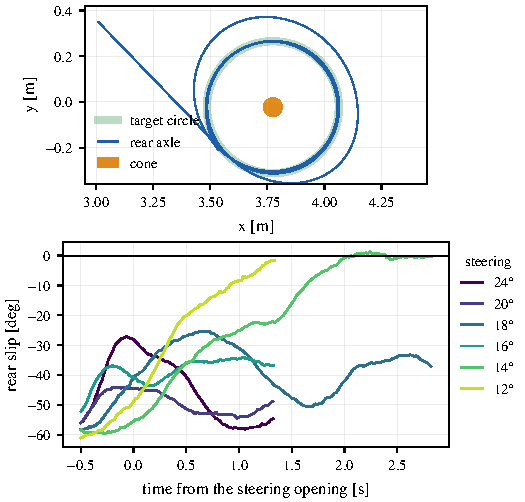
\includegraphics[width=\columnwidth]{figures/drift.pdf}
\caption{Top: Gazebo, the drift NMPC around the cone, true path of the rear axle. Bottom: the car, open loop, rear
slip after the steering opens from the donut at full throttle; it keeps sliding only from \SI{16}{\degree}.}
\label{fig:drift}
\end{figure}

\section{Drift parking}\label{sec:parking}

\subsection{Handbrake turn}

A first parking drove straight, turned, and at a set gyro heading commanded speed zero: the rear wheels lock and
the car slides. Open loop the car stopped anywhere between \SI{177}{\degree} and \SI{197}{\degree}. In the slide
the steering still acts, so every \SI{20}{ms} the node runs the model to the stop for a constant steering and finds,
by bisection, the one that stops the car at the heading asked; the locked rear slides with 1.5 times the friction
of a spinning one. Steered, the stops were \SI{181.6 \pm 2.2}{\degree} over 28 runs. This parking ends nose first:
its body sweeps 40--\SI{50}{cm} behind the stop and needs a gap of about \SI{0.7}{m}.

\subsection{Sideways into a gap}

To park sideways into a tighter gap, the manoeuvre was designed in the refitted model first. Over 6000 random runs
(a straight, one segment of steering and speed, a braked slide) and their local refinement, no run fits in a slot
under \SI{0.47}{m}, 1.8 car lengths: from \SI{0.43}{m/s}, \SI{0.93}{s} at full lock and full throttle, then braked.

The gap node follows that pattern (Fig.~\ref{fig:gap}). At rest it finds the faces of the boxes as a line of
lidar points on its left, and the gap as the break in that line, which also gives the heading to park at. It holds the line of the start at \SI{0.4}{m/s} and kicks where the
predicted stop leaves as much room at the nose as beyond the swept tail: full lock and full throttle, the rear steps
out and the car drifts round at \SIrange{3.4}{4.0}{rad/s}. It then brakes when the gyro heading plus the turn of the
slide after the brake reaches \SI{180}{\degree},
\begin{equation}
\psi_{\text{brake}} + \Delta\psi_{\text{slide}} = \SI{180}{\degree},
\end{equation}
with $\Delta\psi_{\text{slide}} = \SI{36.4}{\degree}$ measured over the closed-loop runs. The gyro reading is
\SI{47}{ms} old when the node reads it, and the node carries it forward with the refitted model and sends the brake
when it is due, between its \SI{20}{ms} steps.

The brake still landed with a delay that varied from run to run: it acted \SIrange{10}{41}{ms} after the command,
\SI{24}{ms} on average, \SIrange{2}{8}{\degree} of heading at these yaw rates. The cause was the firmware, which serviced
the micro-ROS executor every \SI{20}{ms} and took one queued \texttt{/drive} message per pass; serviced every
\SI{5}{ms}, the brake acts \SI{10 \pm 3}{ms} after the command.

Over the closed-loop runs from \SI{0.60}{m} down to \SI{0.47}{m} the car stopped at \SI{180.8 \pm 2.9}{\degree}
(nine runs); Table~\ref{tab:gap} lists the clearances. What limits it now is the slide after the brake itself:
\SIrange{29}{43}{\degree} depending on the floor, \SI{29.5}{\degree} on freshly wiped tiles (the one touch),
\SI{35}{\degree} or \SI{42}{\degree} on used ones, the two modes parting \SI{100}{ms} after the brake. From the yaw
rate, the rest of the turn is known to \SI{1.1}{\degree} only \SI{150}{ms} into the slide, too late for the servo to
correct it.

\begin{figure*}[t]
\centering
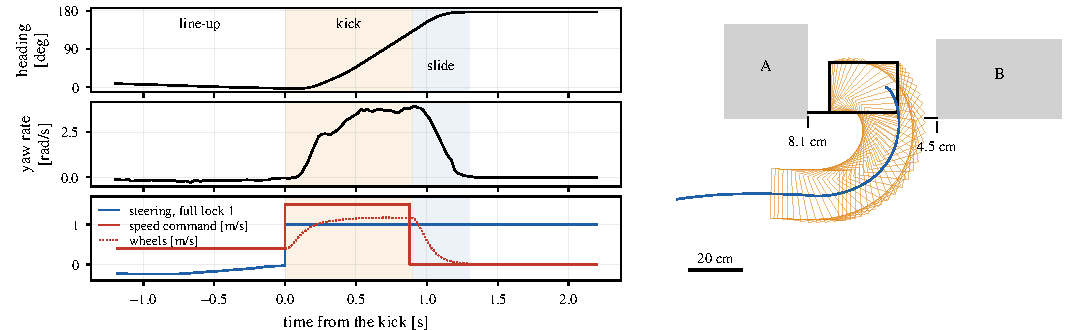
\includegraphics[width=\textwidth]{figures/gap.pdf}
\caption{The parking into the \SI{47}{cm} gap of Fig.~\ref{fig:hero}. Left: heading and yaw rate from the gyro,
and the commands: the line-up at \SI{0.4}{m/s}, the kick at full lock and full throttle, the brake, the slide.
Right: the body every 1/30~s from the kick to the stop, the boxes where the lidar found them, and the closest
approaches.}
\label{fig:gap}
\end{figure*}

\begin{table}[t]
\caption{Gap parking on the tiles, full lock}
\label{tab:gap}
\centering
\footnotesize
\begin{tabular}{@{}rrrr@{}}
\toprule
gap & runs & stop [\si{\degree}] & closest, box A / B [cm] \\
\midrule
\SI{0.60}{m} & 6 & 171.4--183.8 & 7.1--14.2 / 4.0--9.2 \\
\SI{0.54}{m} & 5 & 172.2--183.3 & 2.7--10.9 / 6.4--11.6 \\
\SIrange{0.50}{0.52}{m} & 7 & 176.5--185.5 & 1.9--6.7 / 2.9--8.1 \\
\SI{0.47}{m} & 9 & 173.2--185.7 & 2.5--6.1 / 1.7--6.8 \\
\bottomrule
\end{tabular}
\end{table}

\section{Parking anywhere and the gymkhana}\label{sec:anywhere}

\textbf{Parking anywhere.} Two boxes are put down by hand anywhere in the mapped room. At rest, the lidar points
more than \SI{10}{cm} from the walls of the map are new; two groups of them whose sides towards the car lie on one
line, \SIrange{0.40}{0.75}{m} apart along it, are the boxes and the gap. The parking starts on that line, where the
gap node would start from rest. The approach is the shortest arc--straight--arc path~\cite{dubins1957} of
\SI{0.5}{m} radius that ends on \SI{0.3}{m} of the line with the car's outline \SI{5}{cm} clear of walls and boxes;
when that start cannot be reached driving forward, or when it costs less (a metre backed up counts as two driven),
the path ends further along the line and the gap node backs up first. The NMPC drives the approach
(Fig.~\ref{fig:anywhere}). Over 11 runs with the boxes at six places the car followed the plan within
\SIrange{1.4}{4.8}{cm} rms and stopped between \SI{175.2}{\degree} and \SI{191.4}{\degree}; six runs backed up
\SIrange{0.7}{2.5}{m}, and one touched a box.

\textbf{The gymkhana.} One launch from a start mark chains the nodes, each starting when the one before exits
cleanly: the NMPC drives a lap with a slalom round two cones, the gap node a donut braked on the gyro to end at its
starting heading (it then resets the localization, which the spinning wheels have confused), the NMPC drives back
to the start, and the gap node parks. On the day of the video, under the camera, ten takes were clean\footnote{One more was launched with the car
still parked from the take before, not on its start mark, and drove into a box.}:
\SIrange{28.9}{34.9}{s} each, the lap \SIrange{3.3}{5.6}{cm} rms from its path, the cones at least \SI{8.1}{cm}
from the body, parked at \SIrange{179.3}{182.3}{\degree}, at least \SI{5.4}{cm} from both boxes. Two earlier
takes had stopped on their own: a new node on the Pi found the running ones \SIrange{3}{6}{s} late through DDS
discovery, brought to \SIrange{0.6}{1.5}{s} by sending the discovery announcements more often.

\begin{figure*}[t]
\centering
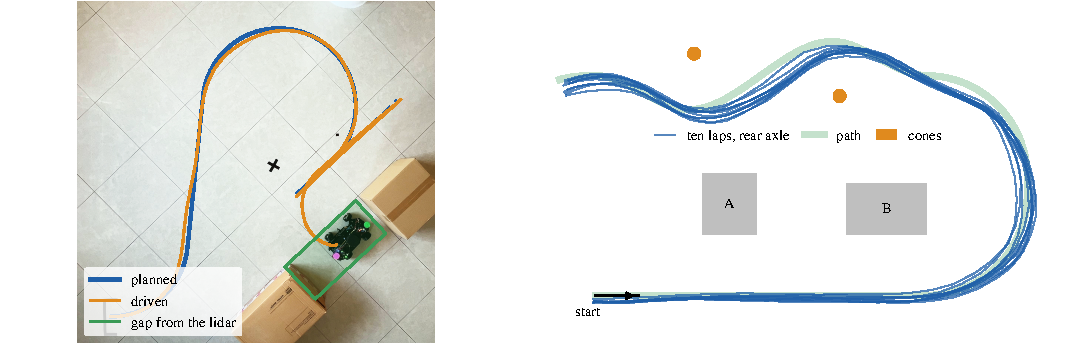
\includegraphics[width=\textwidth]{figures/anywhere.pdf}
\caption{Left: parking anywhere, the boxes at a third place; the path planned from the lidar (blue), which runs
past the gap before the car backs up \SI{0.9}{m} along it, and the path driven by the NMPC (orange), over the
overhead camera at the stop. Right: the slalom lap of
the ten gymkhana takes filmed for the video, rear axle paths from the lidar, with the cones and the boxes.}
\label{fig:anywhere}
\end{figure*}

\section{Simulation twin}\label{sec:sim}

In Gazebo~\cite{koenig2004} a C++ system plugin replaces the ESP32 and the car. It publishes and subscribes the same
topics and integrates the identified model at \SI{1}{kHz} with the measured IMU noise and the brake lag of the
motor driver; the room is built from the map and the lidar is modelled on the A1. The whole stack runs unchanged on
simulated time. With Pure Pursuit it laps in \SI{10.1}{s} as the car does, \SI{4.4}{cm} rms from the line against
\SI{2.7}{cm} on the car: the model turns 4--6\% less in steady corners. The drift replayed open loop gives the same
donut with \SIrange{6}{9}{\degree} more rear slip; the model has no motor torque limit. The twin carried the work
the car could not do safely, friction as a parameter (Sec.~\ref{sec:nmpc}), and the design and debugging of every
node before it ran on the car, including the drift that the car then did not reproduce.

\section{Conclusion}

A low-cost car on hard tires parks itself sideways into a gap of 1.8 car lengths, between boxes it finds itself,
with every computation on board. Three lessons stand out. The model was good enough for an NMPC in grip and for
locked-wheel slides, but not for the transition between grip and drift, and a controller that only works in
simulation can rest on an equilibrium the real system does not have. Delays matter at these yaw rates: a firmware
delay varying between \SI{10}{ms} and \SI{41}{ms} was worth several degrees at the stop, and every sensor needed its
own time base. And
the remaining spread of the parking, a slide that varies by $\pm$\SIrange{3}{4}{\degree} with the state of the floor, is
decided after the brake, where the car can no longer act on it. Natural next steps are an onboard estimate of the
floor friction, which the drift experiments in simulation showed to be observable from the steering, a second
surface, and a faster lidar.

\bibliographystyle{IEEEtran}
\bibliography{refs}

\end{document}
